\documentclass[handout, aspectratio = 169]{beamer}
%\documentclass[presentation]{beamer}

%https://www.overleaf.com/project/5f638086f8e558000137cf72

\usecolortheme{Imperial}
 
\usepackage[utf8]{inputenc}
\usepackage[UKenglish]{babel}
\usepackage{booktabs}
\usepackage{caption}
\usepackage{subcaption}
\usepackage{graphicx}
\usepackage{amsmath}
\usepackage{amsfonts}
\usepackage{amssymb}
\usepackage{epstopdf}
\usepackage{animate}
\usepackage{fancyvrb}

% complying UK date format, i.e. 1 January 2001
\usepackage{datetime}
\let\dateUKenglish\relax
\newdateformat{dateUKenglish}{\THEDAY~\monthname[\THEMONTH] \THEYEAR}

% Imperial College Logo, not to be changed!
\institute{
\includegraphics[height=0.7cm]{Imperial_1_Pantone_solid.eps}}


% -----------------------------------------------------------------------------

\setbeamertemplate{itemize items}[triangle]
\setbeamertemplate{enumerate items}[circle]

%\graphicspath{{figures/}}

%Information to be included in the title page:
\title{Machine Learning Workshop}

%\subtitle{Subtitle}

\author{\color{black} \textbf{Tim C.D. Lucas}\\
{\color{white}blank}\\

\includegraphics[height=7pt]{Ar_Icon_Contact.pdf} tlucas{\footnotesize{@}}ic.ac.uk}

\date{\today}



\begin{document}
 
\frame{\titlepage

% pushes logo up a little but doesn't affect blue line.
\vspace{-0.2cm}
\hfill % pushes logo the right
\includegraphics[width=5cm]{../../ceh_logo.png}

}


% todo
% More pictures.


% new plan:

% overview of analysis and explain each bit.
%   Straight in and do ML.
% What is ML and what is it good for without code.






%1 what is ml 
%what models count
%2 tasks
% famous examples
%4 fit rpart in caret
%- the data
%- hold out
%- error metric
%3 what is caret and it helps an interface with %those many different models


%5 what is ml good at
%compare lm and RF in simplest caret

%6 what is ml bad at
%compare RF and Newton on planets and gravity
%uncertainty

%7 tuning parameters.
%7 very flexible models
%do x^6
%overfitting
%8 bias variance
%9 we might call 6 a hyperparameter.
%lots of models have hyperparameters that %control how regularised the model is.

%10 how do we choose it?
%use hold out data
%CV
%Caret tune parameter

%11 inner outer. use outer for main research %question. which model is best or how well will %my model work in the real world.

%13 match error metric to question


%12 a full machine learning workflow.


%extras:


%14 ask questions with cv
%15-17 trees, RF, enet in a bit more detail. nnet.
%18 no free lunch. try lots of models



% todo



\begin{frame}[fragile]
\frametitle{\insertframenumber~Machine Learning Workshop: Workflow overview.}
\footnotesize{
\vspace{3mm}
{\color{gray}Please open R script lucas\_ml\_workshop.R and load packages.

We'll talk about the following code in a minute.}
\vspace{1mm}
\begin{Verbatim}
tr1 <- trainControl(
         method = 'LGOCV',        # Hold out data for testing
         p = 0.75,
         number = 1,
         savePredictions = TRUE)

m1 <-  train(
	 time ~ .,                # Define response and covariates
         data = melanoma,         # Select the data
         method = 'rpart2',       # Choose a model
         tuneLength = 3,          # Setup fine tuning
         metric = 'MAE',          # Define what counts as `good'
         trControl = tr1)

\end{Verbatim}
}
\end{frame} 




\begin{frame}
\frametitle{\insertframenumber~Workshop structure}
\begin{enumerate}
\item Overview of machine learning workflow/single analysis.
\item Describe data and run basic analysis.
\item What is machine learning?
\item Detailed description of each stage in the analysis.
\item More information on caret.
\item What is machine learning bad at?
\item Fuller machine learning workflow.
\item Final details.
\end{enumerate}

\end{frame} 


\begin{frame}[fragile]
\frametitle{\insertframenumber~ Machine Learning Workshop: Workflow overview.}

\vspace{2mm}
\begin{Verbatim}
tr1 <- trainControl(
         method = 'LGOCV',        # Hold out data for testing
         p = 0.75,
         number = 1,
         savePredictions = TRUE)

m1 <-  train(
	 time ~ .,                # Define response and covariates
         data = melanoma,         # Select the data
         method = 'rpart2',       # Choose a model
         tuneLength = 3,          # Setup fine tuning
         metric = 'MAE',          # Define what counts as `good'
         trControl = tr1)

\end{Verbatim}

\end{frame} 




\begin{frame}[fragile]
\frametitle{\insertframenumber~Let's do Machine Learning: Data}
Time until death data. See script.
\begin{Verbatim}

data(melanoma, package = "boot")
head(melanoma)

# Remove year and discuss censoring.
melanoma <- melanoma[, -5]

# Overview of data.
featurePlot(melanoma[, -1], y = melanoma$time)

\end{Verbatim}

\end{frame} 




\begin{frame}[fragile]
\frametitle{\insertframenumber~ Let's do Machine Learning: Basic analysis}

\vspace{2mm}
\begin{Verbatim}
tr1 <- trainControl(
         method = 'LGOCV',        # Hold out data for testing
         p = 0.75,
         number = 1,
         savePredictions = TRUE)

m1 <-  train(
	 time ~ .,                # Define response and covariates
         data = melanoma,         # Select the data
         method = 'rpart2',       # Choose a model
         tuneLength = 3,          # Setup fine tuning
         metric = 'MAE',          # Define what counts as `good'
         trControl = tr1)

\end{Verbatim}

\end{frame} 






\begin{frame}[fragile]

\small
\begin{Verbatim}
CART 

205 samples
  5 predictor

No pre-processing
Resampling: Repeated Train/Test Splits Estimated (1 reps, 75%) 
Summary of sample sizes: 156 
Resampling results across tuning parameters:

  maxdepth  RMSE      Rsquared   MAE     
  1         890.3811  0.2915851  697.8748
  2         856.7927  0.3493889  687.3165
  3         831.3940  0.3999163  645.2901

MAE was used to select the optimal model using the smallest value.
The final value used for the model was maxdepth = 3.

\end{Verbatim}

\end{frame} 





\begin{frame}
\frametitle{\insertframenumber~Any questions?}

(This slide will occur many times in this slidedeck.)

\end{frame} 












\begin{frame}
\frametitle{\insertframenumber~What is machine learning?}
\begin{itemize}
\item Focus on prediction.
\item Not mechanistic/process based models.
\item Not inference of real-world parameters.
\end{itemize}
\end{frame} 







\begin{frame}
\frametitle{\insertframenumber~What is machine learning?}

\begin{itemize}
\item An analytical aim, rather than a group of models.
\item Linear regression is machine learning if you mostly care about prediction!
\item Also Neural networks, decision trees, random forest.
\end{itemize}

\end{frame} 




\begin{frame}
\frametitle{\insertframenumber~What is machine learning?}
Tasks:
\begin{itemize}
\item Supervised learning
\begin{itemize}
\item Covariates and response data. Like most biological models.
\end{itemize}
\item Reinforcement learning
\begin{itemize}
\item Make your own data.
\end{itemize}
\item Unsupervised learning
\begin{itemize}
\item Clustering.
\end{itemize}
\end{itemize}
\end{frame} 



\begin{frame}
\frametitle{\insertframenumber~What is machine learning?}
Supervised learning.

Classification or regression.
\begin{figure}
    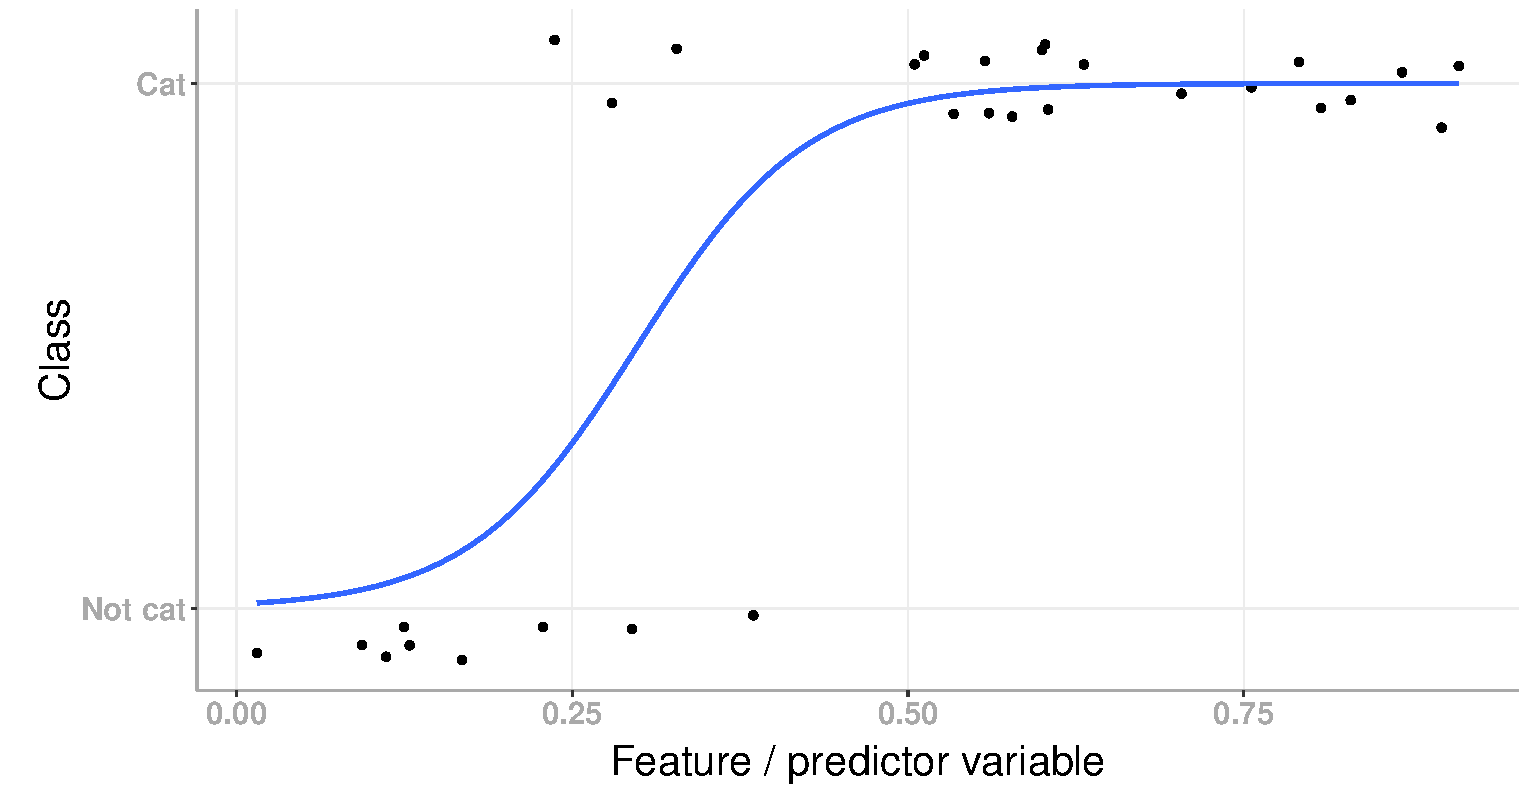
\includegraphics[width = 0.5\textwidth]{classification}%
    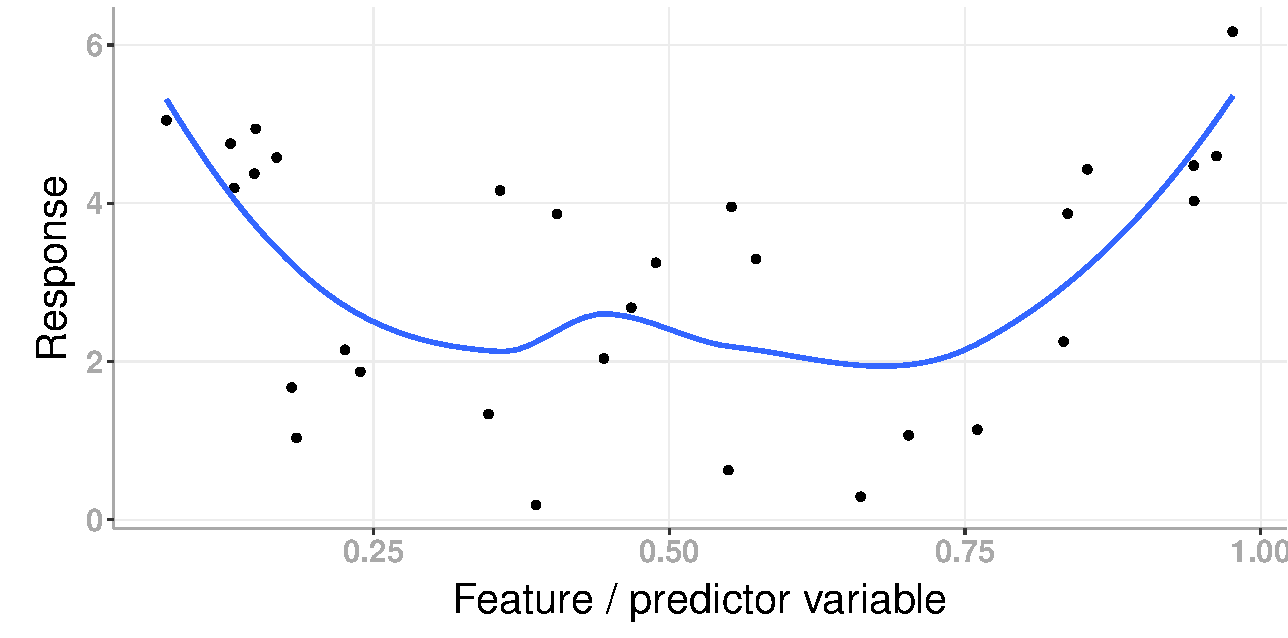
\includegraphics[width = 0.5\textwidth]{regression}
\end{figure} 

\end{frame} 





\begin{frame}
\frametitle{\insertframenumber~Any questions?}


\end{frame} 







\begin{frame}[fragile]
\frametitle{\insertframenumber~ Out-of-sample validation}
\renewcommand{\FancyVerbFormatLine}[1]{%
   \ifnum\value{FancyVerbLine}=2\color{cyan}#1%
   \else #1\fi}
\begin{Verbatim}
tr1 <- trainControl(
        method = 'LGOCV',
        number = 1,
        p = 0.75,
        savePredictions = TRUE)

m1 <- train(time ~ ., 
            data = melanoma,
            method = 'rpart2',
            tuneLength = 3,
            metric = 'MAE',
            trControl = tr1)
            
\end{Verbatim}

\end{frame} 



\begin{frame}
\frametitle{\insertframenumber~Out-of-sample validation}

\begin{itemize}
\item k-fold
\begin{itemize}
\item split into k group. user each group on turn as hold out.
\end{itemize}
\item Repeated k-fold
\begin{itemize}
\item Do k-for multiple times with different random splits.
\end{itemize}
\item Bootstrap
\begin{itemize}
\item Sample N with replacement as training.
\end{itemize}
\end{itemize}
\end{frame} 

\begin{frame}
\frametitle{\insertframenumber~Out-of-sample validation}

\begin{itemize}
\item Seperate study
\item Spatial
\item Temporal
\item By covariates
\item What question do you want to ask?
\end{itemize}
\end{frame} 


\begin{frame}
\frametitle{\insertframenumber~Outer validation}

\begin{itemize}
\item Selecting a model \emph{is part of the model}.
\item If we consider many models, taking the best one is a form of overfitting
\item Outer cross-validation if this is part of primary research question.
\item Unfortunately not implemented in caret. Must do it manually.
\item AKA Train, test, validate.
\end{itemize}
\end{frame} 






\begin{frame}
\frametitle{\insertframenumber~Any questions?}


\end{frame} 





\begin{frame}[fragile]
\frametitle{\insertframenumber~ Let's do Machine Learning: Error metrics.}
\renewcommand{\FancyVerbFormatLine}[1]{%
   \ifnum\value{FancyVerbLine}=11\color{cyan}#1%
   \else #1\fi}
\begin{Verbatim}
tr1 <- trainControl(
        method = 'LGOCV',
        number = 1,
        p = 0.75,
        savePredictions = TRUE)

m1 <- train(time ~ ., 
            data = melanoma,
            method = 'rpart2',
            tuneLength = 3,
            metric = 'MAE',
            trControl = tr1)
            
\end{Verbatim}

\end{frame} 


\begin{frame}
\frametitle{\insertframenumber~Error metrics: regression}

\begin{itemize}
\item Match error metric to question.
\item Aim for interpretability.
\item $MAE = \operatorname{mean}(\operatorname{abs}(\text{pred} - \text{obs})) $
\item $R^2$
\item RMSE, correlation are less interpretable
\item Correlation isn't quite measuring what you think.
\item Scatter plots!
\end{itemize}
\end{frame} 




\begin{frame}
\frametitle{\insertframenumber~Error metrics: regression}

\begin{itemize}
\item Scatter plots!
\item Annoyingly caret doesn't have a function that plots obs vs preds of the hold out data.
\item I have written my own plotCV() function. We'll load it later.
\end{itemize}
\end{frame} 






  \begin{frame}[fragile]
\frametitle{\insertframenumber~Error metrics: regression}

\vspace{5mm}
    \begin{center}
     \includegraphics[width=0.75\textwidth]{scatter_1.pdf}
     \end{center}

\end{frame}




\begin{frame}
\frametitle{\insertframenumber~Error metrics: classification}

\begin{itemize}
\item Match error metric to question.
\item Aim for interpretability.
\item Class balance. Model that never predicts rare class will have high accuracy.
\item I can predict COVID infection with $\sim$97\% accuracy by saying noone has COVID. 
\item Kappa, AUC.
\item Accuracy does *not* account for imbalance.
\item Confusion matrices.
\end{itemize}
\end{frame} 


\begin{frame}
\frametitle{\insertframenumber~Any questions?}


\end{frame} 





\begin{frame}[fragile]
\frametitle{\insertframenumber~Chosing a method (surprisingly unimportant)}
\renewcommand{\FancyVerbFormatLine}[1]{%
   \ifnum\value{FancyVerbLine}=9\color{cyan}#1%
   \else #1\fi}
\begin{Verbatim}
tr1 <- trainControl(
        method = 'LGOCV',
        number = 1,
        p = 0.75,
        savePredictions = TRUE)

m1 <- train(time ~ ., 
            data = melanoma,
            method = 'rpart2',
            tuneLength = 3,
            metric = 'MAE',
            trControl = tr1)
            
\end{Verbatim}

\end{frame} 



\begin{frame}
\frametitle{\insertframenumber~Chosing a method: rpart2}
\vspace{-4mm}
\begin{figure}
    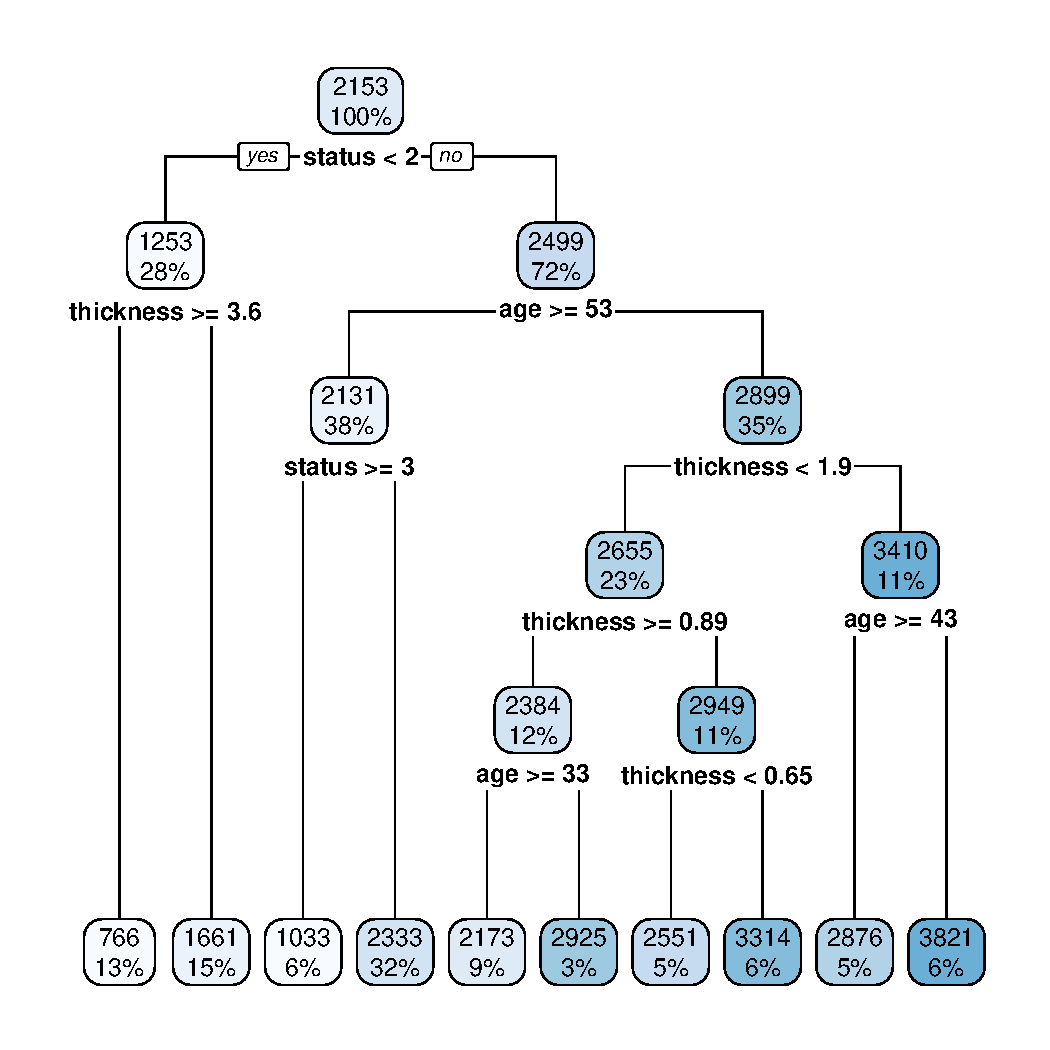
\includegraphics[width = 0.5\textwidth]{rpart_depth6.pdf}
\end{figure} 

\end{frame} 



\begin{frame}
\frametitle{\insertframenumber~No free lunch theorem}
\begin{itemize}
\item No such thing as a universal, `best' machine learning model.
\item So try a few.
\end{itemize}

\end{frame} 



\begin{frame}
\frametitle{\insertframenumber~What is a RandomForest?}

\begin{itemize}
\item method = 'rf' or method = 'ranger' in caret.
\item Instead of 1 tree, fit many trees and take average prediction.
\item For each tree take a random bootstrap of the data.
\item For each node consider a random subset of covariates.
	\begin{itemize}
	\item Consider mtry covariates. Tuning parameter.
	\end{itemize}
\end{itemize}
\end{frame} 


\begin{frame}
\frametitle{\insertframenumber~What is a Neural Network?}

\vspace{6mm}
\begin{figure}
    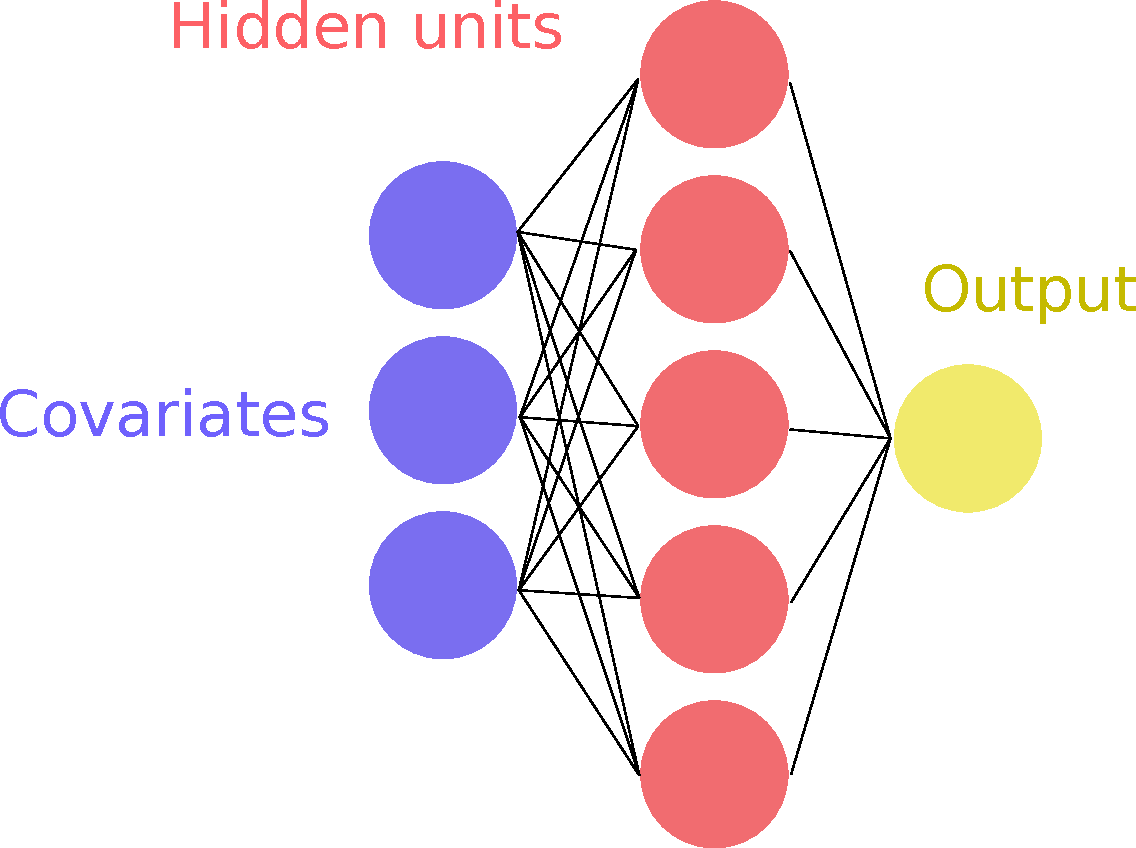
\includegraphics[height = 0.7\textheight]{neural_network.pdf}
\end{figure} 
\end{frame} 


\begin{frame}
\frametitle{\insertframenumber~What is a Neural Network? Little GLMs.}

\vspace{6mm}
\begin{figure}
    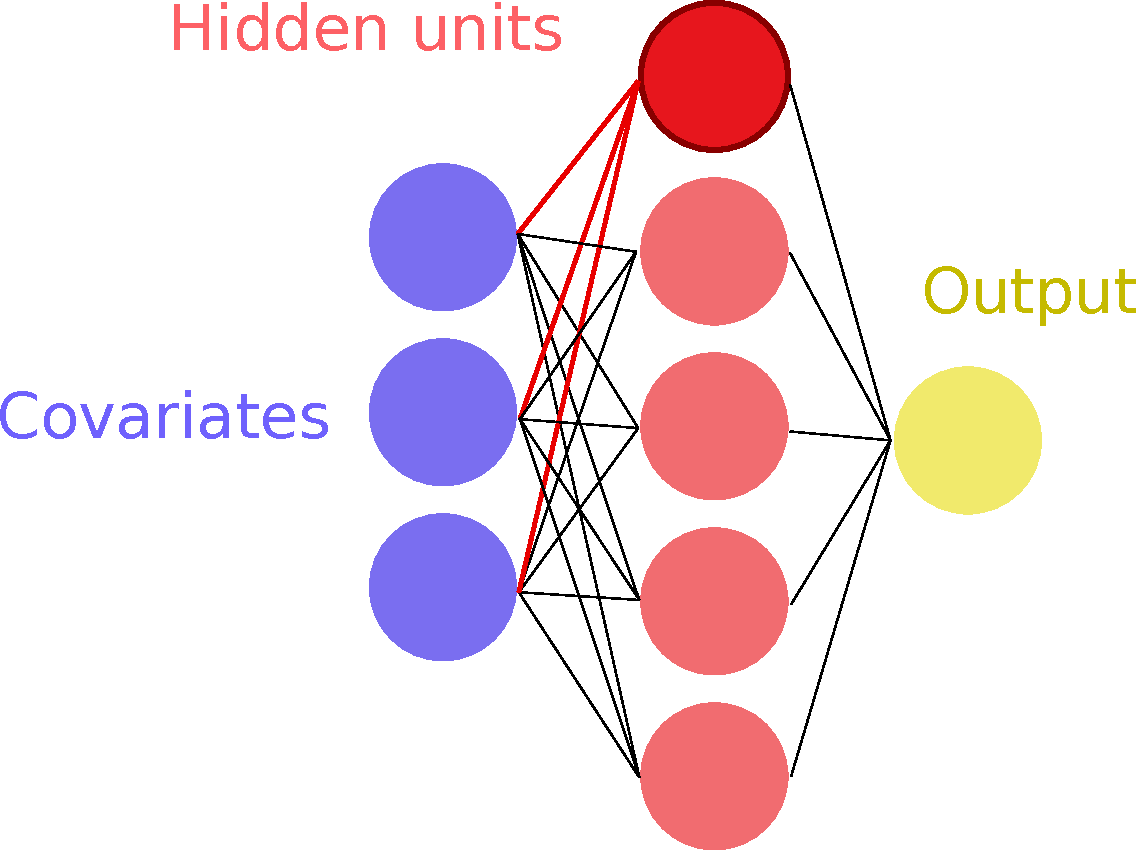
\includegraphics[height = 0.7\textheight]{neural_network2.pdf}
\end{figure} 
\end{frame} 


\begin{frame}
\frametitle{\insertframenumber~What is a Neural Network? Little GLMs.}

\vspace{6mm}
\begin{figure}
    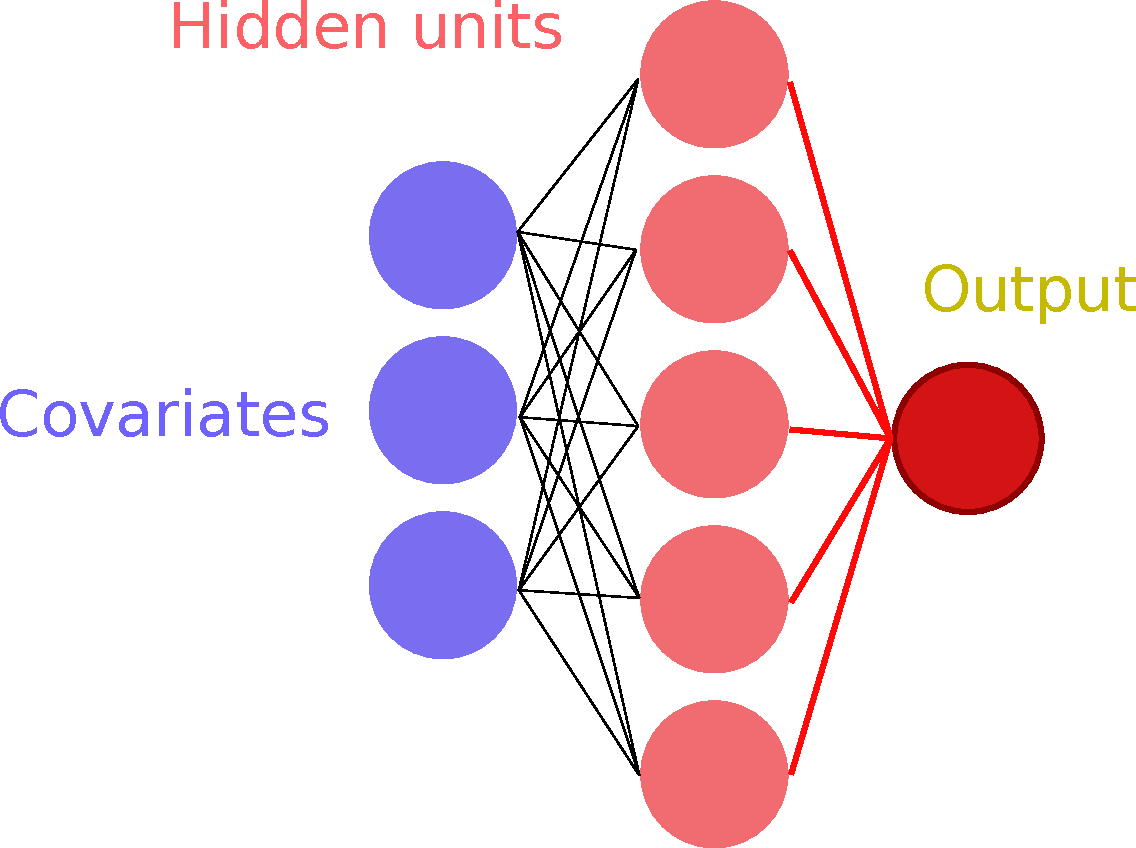
\includegraphics[height = 0.7\textheight]{neural_network3.pdf}
\end{figure} 
\end{frame} 



\begin{frame}
\frametitle{\insertframenumber~What is a Neural Network?}

\begin{itemize}
\item method = 'nnet', method = 'mlpKerasDropout' or many others.
\item Optimise the parameters but there are lots of local optima.
\item What ``architecture''?
	\begin{itemize}
	\item Hidden units.
	\item Extra hidden layers
	\item Everything connected to everything else?
	\end{itemize}
\end{itemize}
\end{frame} 







\begin{frame}
\frametitle{\insertframenumber~Coffee. Any questions?}


\end{frame} 








\begin{frame}[fragile]
\frametitle{\insertframenumber~Tuning/hyperparameters}
\renewcommand{\FancyVerbFormatLine}[1]{%
   \ifnum\value{FancyVerbLine}=10\color{cyan}#1%
   \else #1\fi}
\begin{Verbatim}
tr1 <- trainControl(
        method = 'LGOCV',
        number = 1,
        p = 0.75,
        savePredictions = TRUE)

m1 <- train(time ~ ., 
            data = melanoma,
            method = 'rpart2',
            tuneLength = 3,
            metric = 'MAE',
            trControl = tr1)
            
\end{Verbatim}

\end{frame} 




\begin{frame}
\frametitle{\insertframenumber~Maxdepth parameter}
\vspace{-4mm}
\begin{figure}
    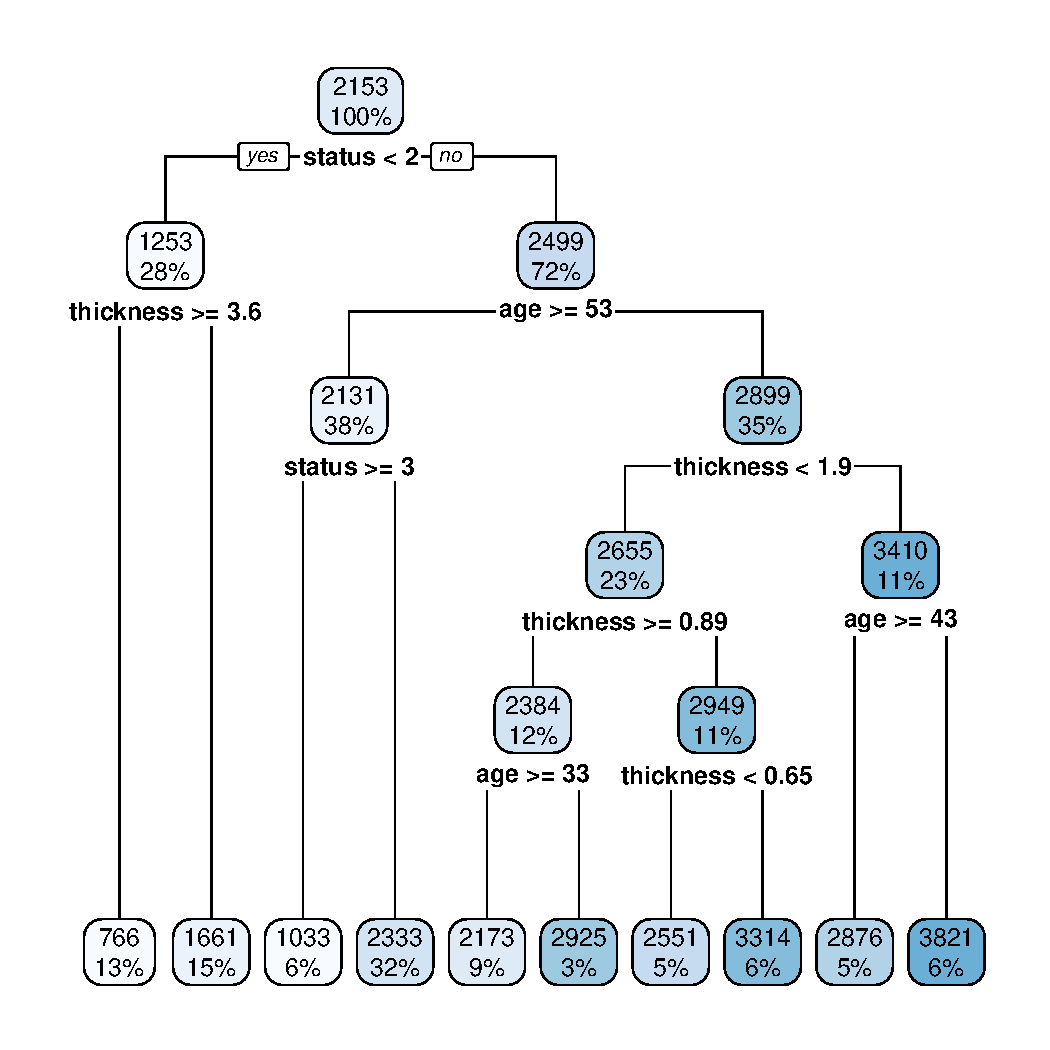
\includegraphics[width = 0.5\textwidth]{rpart_depth6.pdf}
\end{figure} 

\end{frame} 




\begin{frame}
\frametitle{\insertframenumber~Regularisation: forcing a model to be simpler}
\vspace{-4mm}
\begin{figure}
    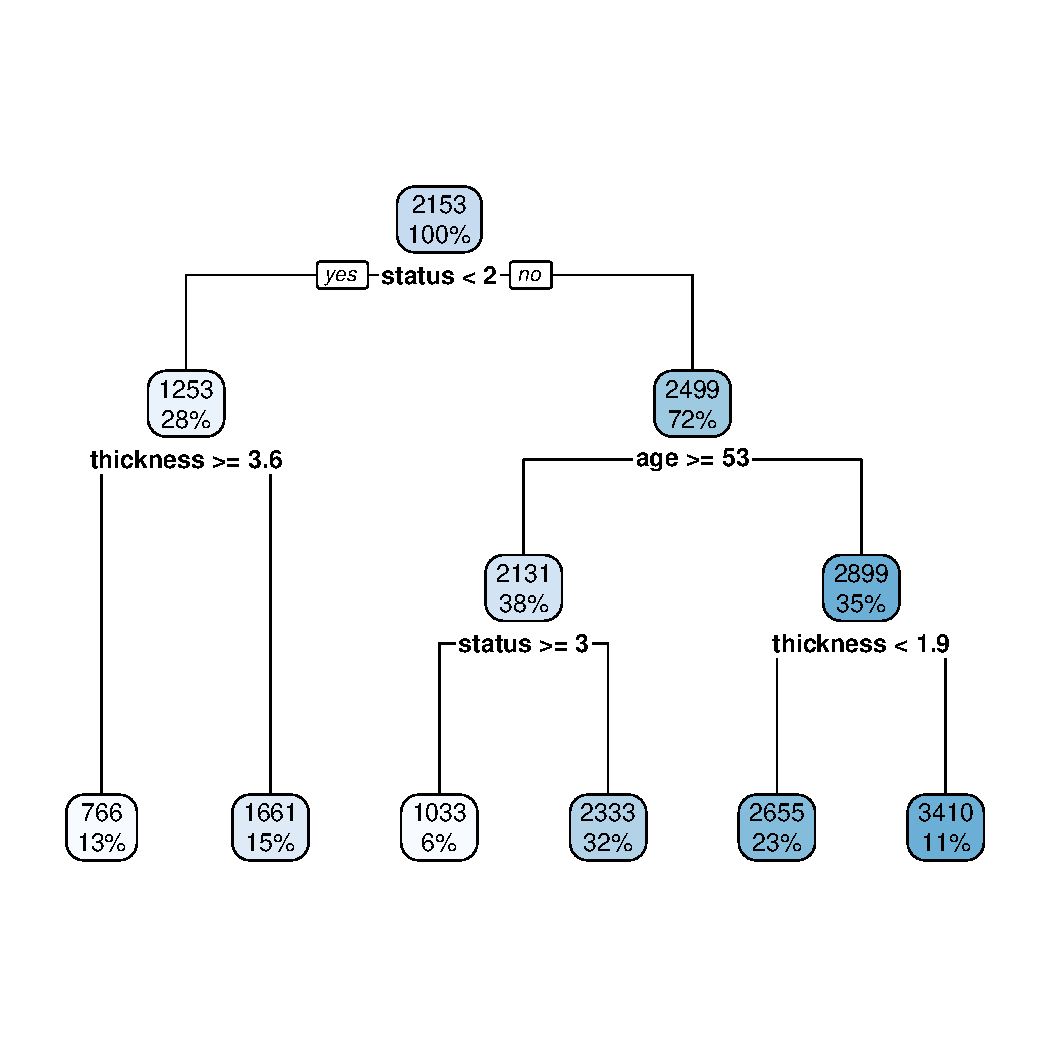
\includegraphics[width = 0.5\textwidth]{rpart_depth3.pdf}
\end{figure} 
\end{frame} 





\begin{frame}
\frametitle{\insertframenumber~How do we choose? Out-of-sample performance.}
\vspace{3mm}
Try \texttt{tuneLength = 10} values.
\vspace{-3mm}
\begin{figure}
    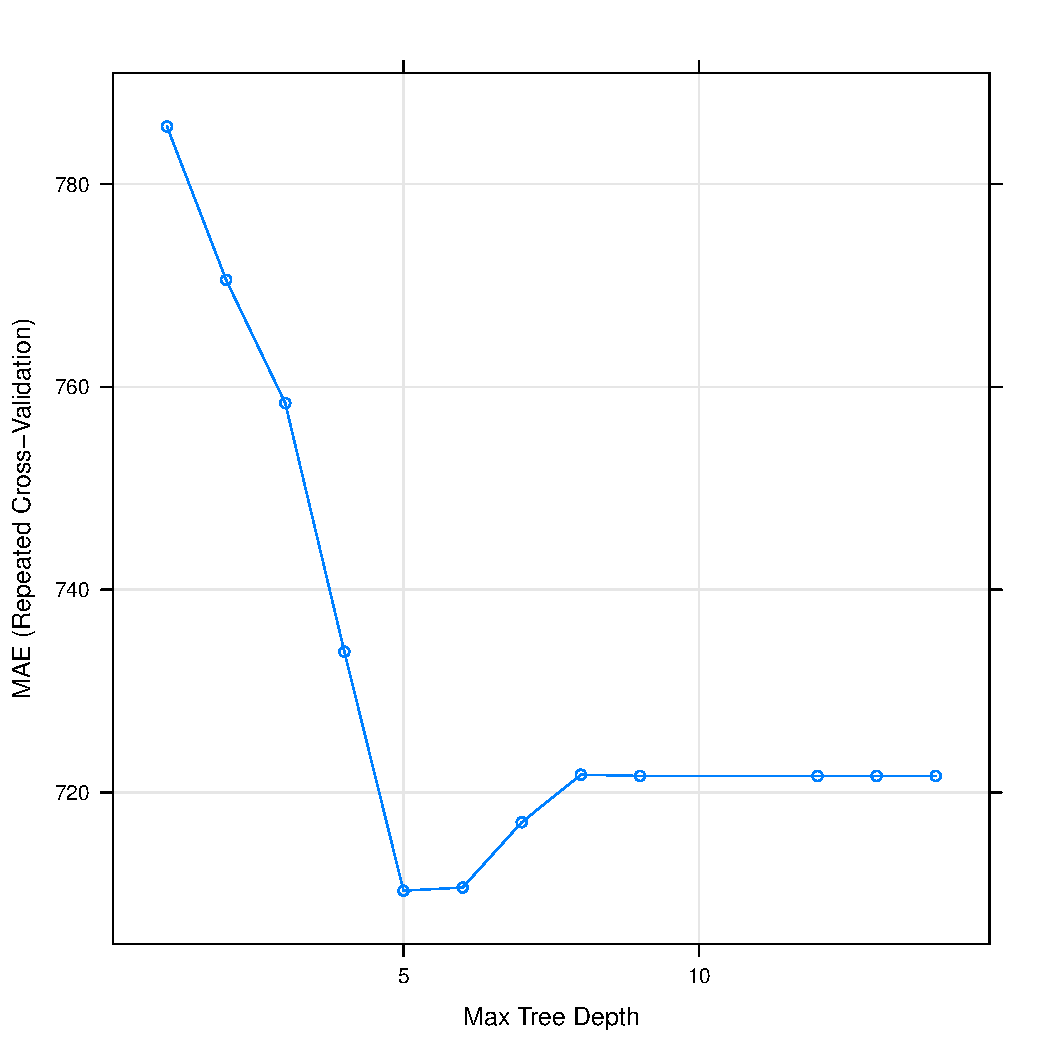
\includegraphics[width = 0.42\textwidth]{rpart_perf.pdf}
\end{figure} 

\end{frame} 


\begin{frame}
\frametitle{\insertframenumber~Other tuning parameters.}
\begin{itemize}
\item Stepwise regression cutoff.
\item Degree of freedom in GAM.
\item Length scale in Gaussian Process.
\item Variance of zero-mean Bayesian prior.
\end{itemize}

\end{frame} 


\begin{frame}
\frametitle{\insertframenumber~Why does error  increase  with model complexity?}
\vspace{-4mm}
\begin{figure}
    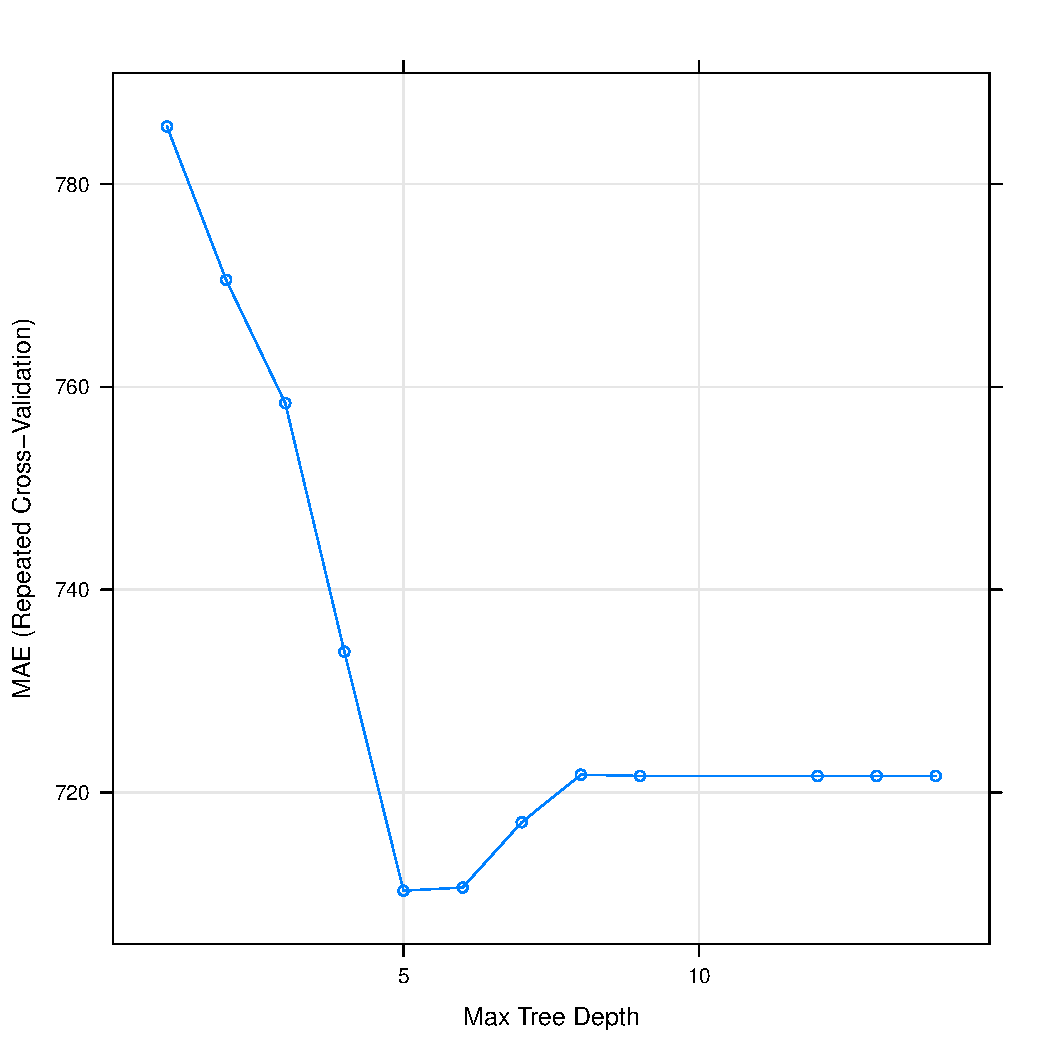
\includegraphics[width = 0.45\textwidth]{rpart_perf.pdf}
\end{figure} 

\end{frame} 


\begin{frame}
\frametitle{\insertframenumber~Overfitting and bias/variance.}

\begin{figure}
    \includegraphics[height = 0.8\textheight]{bias_variance.pdf}
\end{figure} 

\end{frame} 


\begin{frame}
\frametitle{\insertframenumber~Overfitting and bias/variance.}

\begin{figure}
    \includegraphics[height = 0.8\textheight]{bias_variance_optim.pdf}
\end{figure} 

\end{frame} 



\begin{frame}
\frametitle{\insertframenumber~Any questions?}


\end{frame} 

































\begin{frame}
\frametitle{\insertframenumber~Caret package}
\begin{itemize}
\item https://topepo.github.io/caret/model-training-and-tuning.html
\item Unified interface to hundreds of models
\item Supervised learning
\item Full ML workflow
\item Excellent documentation


\end{itemize}

\end{frame} 


\begin{frame}
\frametitle{\insertframenumber~Caret details}
\begin{enumerate}
\item Fit model to all training sets and predict all test sets with all hyperparameter combinations.
\item Select best hyperparameter combination.
\item Fit model using best hyperparameter set to all data.
\item If y is a factor, automatically do classification.
\item Some models are only regression, some only classification, some both.
\item Caret will ask you if you want to install additional packages.
\item Some models don't handle NAs. Error messages not always very useful.
\item Check documentation for parallel computation.
\end{enumerate}

\end{frame} 



\begin{frame}
\frametitle{\insertframenumber~Caret documentation}

\begin{itemize}
\item https://topepo.github.io/caret/index.html
\item Really excellent!
\item Model list with tuning parameters.
\item Models by tag (data weights, tree-based, implicit feature selection).
\end{itemize}
\end{frame} 




\begin{frame}[fragile]
\frametitle{\insertframenumber~Caret functions and internals}
\begin{Verbatim}

plot(m1)

# Uses model trained on full dataset.
# Use this to test on a outer validation dataset.
predict(m1) 

m1$results # Validation results.
m1$pred # All validation predictions (all hyperpars)
m1$finalModel # The final fitted model
class(m1$finalModel)


\end{Verbatim}

\end{frame} 






\begin{frame}[fragile]
\frametitle{\insertframenumber~Caret functions and internals}
\begin{Verbatim}

# Load plotCV() and best_tune_preds() functions.

plotCV(m1) 

\end{Verbatim}

\end{frame} 




\begin{frame}[fragile]
\frametitle{\insertframenumber~Grid search for models with many hyperparameters}
\begin{Verbatim}

tr_random <- trainControl(
              search = 'random',
              savePredictions = TRUE)

m_random <- train(time ~ ., 
            data = melanoma,
            method = 'enet',
            tuneLength = 20,
            metric = 'MAE',
            trControl = tr_random)
            
\end{Verbatim}

\end{frame} 




\begin{frame}[fragile]
\frametitle{\insertframenumber~Grid search for models with many hyperparameters}
\begin{Verbatim}

# Give an explit dataframe of parameters
# Need to look up the exact names 

gr <- data.frame(lambda = c(1e-4, 1e-5, 1e-6),
                 fraction = c(0.1, 0.5, 0.5))
m_df <- train(time ~ ., 
            data = melanoma,
            method = 'enet',
            tuneGrid = gr,
            metric = 'MAE',
            trControl = tr1)
plot(m_df)

            
\end{Verbatim}

\end{frame} 



\begin{frame}
\frametitle{\insertframenumber~Any questions?}


\end{frame} 










\begin{frame}[fragile]
\frametitle{\insertframenumber~What is ML bad at?}
\renewcommand{\FancyVerbFormatLine}[1]{%
   \ifnum\value{FancyVerbLine}=1\color{cyan}#1%
   \else #1\fi}
\begin{Verbatim}
pl <- read.csv(
  file = 'https://raw.githubusercontent.com/timcdlucas/ml_workshop/master/planets.csv')

pl1 <- train(g ~ ., 
            data = pl,
            method = 'rpart2',
            trControl = tr1)


\end{Verbatim}

\end{frame} 


\begin{frame}[fragile]
\frametitle{\insertframenumber~What is ML bad at?}
\renewcommand{\FancyVerbFormatLine}[1]{%
   \ifnum\value{FancyVerbLine}=1\color{cyan}#1%
   \else #1\fi}
\begin{Verbatim}
pl <- read.csv(
  file = 'https://raw.githubusercontent.com/timcdlucas/ml_workshop/master/planets.csv')

pl2 <- train(g ~ 0 + I(m1 * m2 / d ^ 2), 
            data = pl,
            method = 'lm',
            trControl = tr1)

\end{Verbatim}

\end{frame} 



\begin{frame}
\frametitle{\insertframenumber~Which was better? Any questions?}

\begin{itemize}
\item Thumbs up: rpart2.
\item Smiley face: lm.
\end{itemize}
\end{frame} 






\begin{frame}
\frametitle{\insertframenumber~Short coffee.}


\end{frame} 










\begin{frame}[fragile]
\frametitle{\insertframenumber~Fuller ML workflow}
\begin{Verbatim}

# Carefully think about hold out data
# This is THE most important part.
tr2 <- trainControl(
        method = 'repeatedcv',
        number = 5,
        repeats = 3, 
        savePredictions = TRUE)


\end{Verbatim}

\end{frame} 


\begin{frame}[fragile]
\frametitle{\insertframenumber~Fuller ML workflow}
\begin{Verbatim}

# Carefully choose a metric
my_metric <- 'MAE'

\end{Verbatim}

\end{frame} 

	

\begin{frame}[fragile]
\frametitle{\insertframenumber~Fuller ML workflow}
\begin{Verbatim}

# Collect data.
# Make new covariates. GDP growth, sum of air pollution last week.
# Covariates are more important than algorithms.

# Log, sqrt, sqaured for linear models.
# Tree models focus on combining covariates.


\end{Verbatim}

\end{frame} 



\begin{frame}[fragile]
\frametitle{\insertframenumber~Fuller ML workflow}
\begin{Verbatim}

# Baseline linear model
m1 <- train(time ~ ., 
            data = melanoma,
            method = 'enet',
            tuneLength = 10,
            metric = my_metric,
            trControl = tr2)


# Look at scatter plots for regression
# Look at confusion matrix for classification
plotCV(m1)

\end{Verbatim}

\end{frame} 



\begin{frame}[fragile]
\frametitle{\insertframenumber~Fuller ML workflow}
\begin{Verbatim}

# Projection pursuit regression is very fast but nonlinear.
#   Another good baseline.
m2 <- train(time ~ ., 
            data = melanoma,
            method = 'ppr',
            tuneLength = 10,
            metric = my_metric,
            trControl = tr2)


# Look at scatter plots for regression
plotCV(m2)

\end{Verbatim}

\end{frame} 


\begin{frame}[fragile]
\frametitle{\insertframenumber~Fuller ML workflow}
\begin{Verbatim}

# Random Forest often peforms very well.
# Easy to tune. Another excellent baseline.
m3 <- train(time ~ ., 
            data = melanoma,
            method = 'ranger',
            tuneLength = 5,
            metric = my_metric,
            trControl = tr2)

plotCV(m3)
pdp::partial(m3, pred.var = c('thickness'), plot = TRUE)

\end{Verbatim}

\end{frame} 


\begin{frame}
\frametitle{\insertframenumber~Partial dependence plot.}
\vspace{2mm}
Fitted relationship between thickness and time.
\begin{figure}
    \includegraphics[width = 0.4\textwidth]{rf_pdp_1.pdf}

\end{figure} 

\end{frame} 



\begin{frame}[fragile]
\frametitle{\insertframenumber~Fuller ML workflow}
\vspace{1mm}
\begin{Verbatim}
tr2_random <- trainControl(
        method = 'repeatedcv',
        number = 5,
        repeats = 3, 
        search = 'random',
        savePredictions = TRUE)

m4 <- train(time ~ ., 
            data = melanoma,
            method = 'xgbTree',
            tuneLength = 10,
            metric = my_metric,
            trControl = tr2)

\end{Verbatim}

\end{frame} 


\begin{frame}[fragile]
\frametitle{\insertframenumber~Fuller ML workflow}
\begin{Verbatim}

# Try a few models. No free lunch.
m5 <- train(time ~ ., 
            data = melanoma,
            method = 'nnet',
            tuneLength = 10,
            metric = my_metric,
            linout = TRUE,
            trControl = tr2)

# Neural networks need linout = TRUE for regression.
# linear output as apposed to logit/probit.

\end{Verbatim}

\end{frame} 



\begin{frame}
\frametitle{\insertframenumber~Any questions?}


\end{frame} 





\begin{frame}
\frametitle{\insertframenumber~Other packages}

\begin{itemize}
\item mlr3
	\begin{itemize}
	\item I find it more complicated. 
	\item Probably better for very complicated pipelines.
	\end{itemize}
\item tidymodels
	\begin{itemize}
	\item Fits into tidyverse.
	\item More complicated.
	\item Not yet feature complete.
	\end{itemize}
\item scikit.learn in Python
\item caretEnsemble for ensembles/model averaging.
\end{itemize}
\end{frame} 




\begin{frame}
\frametitle{\insertframenumber~Extra reading}

\begin{itemize}
\item Breiman 2001 Statistical Modeling: The Two Cultures.
\item Molnar 2020 Interpretable Machine Learning: A Guide for Making Black Box Models Explainable.
\item Kuhn 2013 Applied Predictive Modeling.
\item Lucas 2020 A translucent box: interpretable machine learning in ecology.
\item Bhatt et al. 2017 Improved prediction accuracy for disease risk mapping using Gaussian process stacked generalization
\end{itemize}
\end{frame} 




\begin{frame}

\frametitle{\insertframenumber~Any questions?}

\vspace{5mm}


\vspace{4mm}


\includegraphics[height=7pt]{Ar_Icon_Contact.pdf} tlucas{\footnotesize{@}}ic.ac.uk


\includegraphics[height=7pt]{Twitter_logo_blue-small.png} {\footnotesize{@}}StatsForBios

\vspace{2cm}
\hfill % pushes logo the right
\includegraphics[width=5cm]{../../ceh_logo.png}

\end{frame}


%thanks


 
 
\end{document}


